\chapter{Concept Assessment}\label{cha:assessment}

    The assessment of this project is calculated based on the number of interaction and complexity levels achieved as described in Tables~\ref{tab:uilevels} and~\ref{tab:techlevels}. Illustrated in Table~\ref{tab:levelCompare} is the relation between the level of user interaction and the technical complexity. The blue dots indicate the complexity level required to achieve a specific level of interaction. For example, interaction level $\mathcal{I}4$ (intermediate) requires a complexity of $\mathcal{C}5$ in order to be implemented. The highlighted section denotes the completed objectives for this project.

    \newcommand{\bmark}{\hskip 0.5em $\color{igmrBlue}\bullet$ \hskip 0.5em}
    \newcommand{\nomark}{\hskip 0.5em $\color{shade30}\circ$ \hskip 0.5em}
    \newcommand{\cshade}{\cellcolor{shade10}}

    \begin{table}[htbp]
        \color{textColor}
        \centering	
        \begin{tabular}{ cr|cccccccccc }
             &&&&&&&&&& \\
            \multirow{8}{*}{\rotatebox[origin=c]{90}{Interaction $[\,\mathcal{I}\,]\ \longrightarrow$\ }} 

             & $\mathcal{I}6$ & \bmark & \bmark & \bmark & \bmark & \bmark & \bmark & \bmark & \bmark & \bmark & \\[1em]

             & $\mathcal{I}5$ & \bmark & \bmark & \bmark & \bmark & \bmark & \bmark & \bmark & \nomark & \nomark & \\[1em]

             & $\mathcal{I}4$ & \cshade \bmark & \cshade \bmark & \cshade \bmark & \cshade \bmark & \cshade \bmark & \nomark & \nomark & \nomark & \nomark & \\[1em]

             & $\mathcal{I}3$ & \cshade \bmark & \cshade \bmark & \cshade \bmark & \cshade \nomark & \cshade \nomark & \nomark & \nomark & \nomark & \nomark & \\[1em]

             & $\mathcal{I}2$ & \cshade \bmark & \cshade \bmark & \cshade \nomark & \cshade \nomark & \cshade \nomark & \nomark & \nomark & \nomark & \nomark & \\[1em]

             & $\mathcal{I}1$ & \cshade \bmark & \cshade \bmark & \cshade \nomark & \cshade \nomark & \cshade \nomark & \nomark & \nomark & \nomark & \nomark & \\[1em]
             
            \cline{2-11} 
             &&&&&&&&&& \\[-5pt]
             &  & $\mathcal{C}1$ & $\mathcal{C}2$ & $\mathcal{C}3$ & $\mathcal{C}4$ & $\mathcal{C}5$ & $\mathcal{C}6$ & $\mathcal{C}7$ & $\mathcal{C}8$ & $\mathcal{C}9$ & \\[0.5em]
             &  \multicolumn{10}{c}{Complexity $[\,\mathcal{C}\,]\ \longrightarrow$} \\
        \end{tabular}
        \caption{Relation between user interaction and increasing technical complexity.}
        \label{tab:levelCompare}
    \end{table}

    It is assumed that users  will vary depending on the application. A beginner user, $\mathcal{U}1$, will benefit from an intermediate interface, $\mathcal{I}4$, when learning \ac{ROS} concepts. However, a student with programming experience, $\mathcal{U}2$, will demand a more interactive \ac{ROS} playground, $\mathcal{I}5$ and above. Similarly, experienced users, $\mathcal{U}3$ and $\mathcal{U}4$ will require all \ac{ROS} tools to be available, $\mathcal{I}6$, to justify a migration to a web browser platform.

\section{Layer Progression}

    The following sections describe the chronological progression of layers to achieve the results highlighted with gray in Table~\ref{tab:levelCompare}. As observed in the table, the progression through the levels is not a linear path, but a series of zigzag steps in multiple directions.

    \vspace{1em}
    \begin{tcolorbox}[title=Note]
        \begin{minipage}[t]{0.87\linewidth}
            \vspace*{0pt}
            If the reader would like to follow along with the demonstrations
            provided in the following pages, it is recommended to visit 
            \href{https://ros2wasm.dev/}{\textsf{ros2wasm.dev}}.
            Throughout the text, links will be provided to redirect the reader 
            to specific examples.
        \end{minipage}\hfill%
        \begin{minipage}[t]{0.1\linewidth}
            \vspace*{0pt}
            
\includegraphics[height=\linewidth,width=\linewidth]{qr_ros2wasm.png}
        \end{minipage}
    \end{tcolorbox}


        \subsection{Complexity Level 1}

        The groundwork for achieving any sort of user interface with \ac{ROS} running on the browser, lies on the development of a compatible middleware implementation ($\mathcal{C}1$). The design of this middleware implementation has been described in Chapter~\ref{cha:rmw}. The three packages (\textsf{rmw-wasm-cpp}, \textsf{wasm-cpp}, and \textsf{wasm-js}) on their own, do not aid the user in interacting with \ac{ROS}.

        \vspace{0.5em}
        \begin{tcolorbox}[title=Example 1]
            \begin{minipage}[t]{0.87\linewidth}
                \vspace*{0pt}
                The source code for the custom middleware implementation packages can be found in the following repository:

                \href{https://github.com/ihuicatl/rmw_wasm/}{\textsf{https://github.com/ihuicatl/rmw\smallunderscore wasm/}}
            \end{minipage}\hfill%
            \begin{minipage}[t]{0.1\linewidth}
                \vspace*{0pt}
                
\includegraphics[height=\linewidth,width=\linewidth]{qr_rmw_wasm.png}
            \end{minipage}
        \end{tcolorbox}

        \subsection{Complexity Level 2}

        The next step in complexity, $\mathcal{C}2$, involves creating a \ac{ROS} package for testing and cross-compiling such package along with its dependencies. For simplicity, the test package follows the official \ac{ROS} tutorials for how to create a publisher and a subscriber that communicate with each other in C++~\cite{humbletutorial}. By having this standard baseline, this ensures that the behavior of the middleware implementation packages can be adjusted until it matches the expected behavior for a typical \ac{ROS} publisher and subscriber. The CMake instructions were modified for each executable in order to have a successful cross-compilation with Emscripten. 

        \vspace{0.5em}
        \begin{tcolorbox}[title=Example 2]
            \begin{minipage}[t]{0.87\linewidth}
                \vspace*{0pt}
                The testing package, \textsf{test-wasm}, used for this project can be found in the following repository:

                \href{https://github.com/ihuicatl/rmw_wasm/tree/main/test_wasm}{\textsf{https://github.com/ihuicatl/rmw\smallunderscore wasm/tree/main/test\smallunderscore wasm}}
            \end{minipage}\hfill%
            \begin{minipage}[t]{0.1\linewidth}
                \vspace*{0pt}
                
\includegraphics[height=\linewidth,width=\linewidth]{qr_test_wasm.png}
            \end{minipage}
        \end{tcolorbox}

        To replicate the process locally, a build script (\textsf{blasm}) is provided in Appendix~\ref{sec:apxblasm}. As prerequisites, it is necessary to have an active installation of Emscripten and a copy of the \ac{ROS} 2 source code in a workspace. Figure~\ref{fig:vcs} shows the recommended procedure for cloning all \ac{ROS} 2 packages by using a \ac{VCS} tool~\cite{rosinstall}.

        \begin{figure}[htbp]
            \centering
            \begin{lstlisting}[language=Bash]
cd ~/workspace/src
vcs import --input https://raw.githubusercontent.com/ros2/ros2/humble/ros2.repos .
\end{lstlisting}
            \caption{Cloning all \ac{ROS} 2 packages with \textsf{vcstool}.}
            \label{fig:vcs}
        \end{figure}

        An even simpler solution for new users to build packages is to use a GitHub workflow. An example of such workflow is given in Appendix~\ref{sec:apxworkflow}. By adding this script to a repository which includes the desired \ac{ROS} package to be built, the user can manually trigger this workflow to build the target package without the need to have a local build set up. Figure~\ref{fig:workflow} displays the interface for running the \textsf{build-package} workflow from GitHub.

        \begin{figure}[htbp]
            \centering
            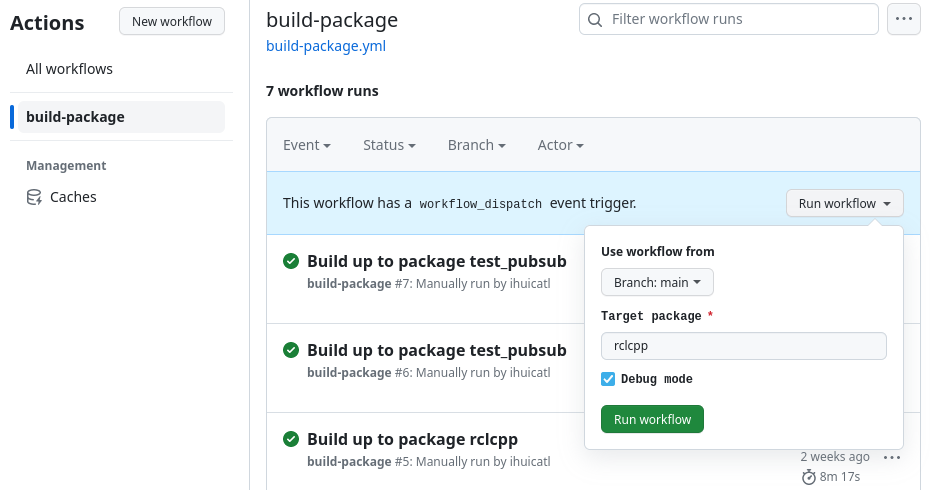
\includegraphics[width=\textwidth]{07_workflow.png}
            \caption{Triggering \textsf{build-package} workflow to build \textsf{rclcpp}.}
            \label{fig:workflow}
        \end{figure}

        \pagebreak

        The workflow runs through the following steps:

        \begin{enumerate}
            \item Install and activate \ac{emsdk}.
            \item Create a \ac{ROS} workspace.
            \item Install \textsf{vcstool}.
            \item Clone all \ac{ROS} 2 packages to the workspace.
            \item Removes unsupported packages such as the default middleware implementations, e.g. \textsf{FastRTPS}.
            \item Applies a patch to \textsf{rcutils} package.
            \item Creates a \textsf{conda} environment with the \textsf{colcon} packages installed.
            \item Runs the \textsf{blasm} script to build up to the target package.
            \item And uploads the artifacts.
        \end{enumerate}

        It is important to note that the artifacts are available for the user to download once the workflow has completed successfully. The contents of these artifacts will include any \ac{WASM}, JavaScript, and \ac{HTML} files generated by the target package during the build. However, the target package must contain executables in order for these files to be generated in the first place.

        This \textsf{build-package} workflow provides an overview of the procedure required to build packages locally or on an external server. Although the initial setup may seem laborious, automation tools can greatly simplify the process. 

        \vspace{0.5em}
        \begin{tcolorbox}[title=Example 3]
            \begin{minipage}[t]{0.87\linewidth}
                \vspace*{0pt}
                The source code for the described workflow can be found in the following repository:

                \href{https://github.com/ihuicatl/ros2wasm/blob/main/.github/workflows/build-package.yml}{\footnotesize{\textsf{https://github.com/ihuicatl/ros2wasm/blob/main/.github/workflows/build-package.yml}}}

                The reader is encouraged to fork the repository to test the workflow.
            \end{minipage}\hfill%
            \begin{minipage}[t]{0.1\linewidth}
                \vspace*{0pt}
                
\includegraphics[height=\linewidth,width=\linewidth]{qr_workflow.png}
            \end{minipage}
        \end{tcolorbox}

        \subsection{User Interaction Level 1: Non-Interactive}

        Once $\mathcal{C}1$ and $\mathcal{C}2$ levels are completed, this opens the door for minimal user interaction. With the testing package described above containing a publisher derived from the \ac{ROS} tutorials, a \ac{WASM} and a JavaScript are generated when cross-compiling the publisher executable. By creating a bare bones \ac{HTML} page, the publisher (\textit{talker}) can be run on the browser.

        \begin{figure}[htbp]
            \begin{lstlisting}[language=html]
<!DOCTYPE html>
<html lang="en">
    <head>
        <meta charset="utf-8">
        <title>Non-Interactive Publisher</title>
        <link rel="stylesheet" href="style.css">
        <script src="wasm_js/rosMain.js"></script>
        <script src="talker.js"></script>
    </head>

    <body>
        <textarea id="talkerOutput"  rows="10"></textarea>
    </body>
</html>
\end{lstlisting}
            \caption{Minimal \ac{HTML} page to run a publisher node on the browser.}
            \label{fig:html}
        \end{figure}

        As indicated in Figure~\ref{fig:html}, the \textit{talker} depends on \textsf{wasm-js} for handling messages and to display outputs on the page. Alternatively, these outputs can also be observed from the console. It is important to note that at this complexity level, $\mathcal{C}2$, \textsf{wasm-js} does not need to be fully equipped; it suffices to receive a \ac{YAML} string message from the publisher node and to display the information on the page. Since there are no subscriber nodes, messages can be discarded automatically.
        
        This type of setup constitutes $\mathcal{I}1$ or non-interactive. The user has no control of the publisher node other than reloading the page to restart the publisher. The output from a publisher in this level is seen in Figure~\ref{fig:ui1}. 

        \begin{figure}[htbp]
            \centering

            \begin{lstlisting}[language=Bash]
Publisher initializing.
[INFO] [1682069093.833000000] [wasm_cpp]: Context initializing.
[INFO] [1682069094.864000000] [wasm_publisher]: Publishing: 'Hello there! 0'
[INFO] [1682069095.877000000] [wasm_publisher]: Publishing: 'Hello there! 1'
[INFO] [1682069096.894000000] [wasm_publisher]: Publishing: 'Hello there! 2'
[INFO] [1682069097.906000000] [wasm_publisher]: Publishing: 'Hello there! 3'
[INFO] [1682069098.922000000] [wasm_publisher]: Publishing: 'Hello there! 4'
[INFO] [1682069099.940000000] [wasm_publisher]: Publishing: 'Hello there! 5'
\end{lstlisting}
            \caption{Output from non-interactive $\mathcal{I}1$.}\label{fig:ui1}
        \end{figure}

        \vspace{2em}
        \begin{tcolorbox}[title=Example 4]
            \begin{minipage}[t]{0.87\linewidth}
                \vspace*{0pt}
                A demonstration of a \textit{non-interactive} user interface ($\mathcal{I}1$) can be found at
                
                \href{https://ros2wasm.dev/pages/demo01/index.html}{\textsf{ttps://ros2wasm.dev/pages/demo01/index.html}}

                \textsc{Note:} The page must be reloaded to restart the node.
            \end{minipage}\hfill%
            \begin{minipage}[t]{0.1\linewidth}
                \vspace*{0pt}
                
\includegraphics[height=\linewidth,width=\linewidth]{qr_demo01.png}
            \end{minipage}
        \end{tcolorbox}

        \subsection{User Interaction Level 2: Minimal}

        With the addition of buttons and the introduction of web workers to the \textsf{wasm-js} middleware package, the user gains the bare minimum control over the publisher node. At this point, the user can only start and stop the node. And as stated previously, without subscribers there is no need for persistent message storage. Figure~\ref{fig:ui2} illustrates this \textit{minimal} user interface, $\mathcal{I}2$.

        \vspace{1em}
        \begin{figure}[htbp]
            \centering
            % 
\includegraphics[width=\linewidth]{03_level2.png}
            \begin{tikzpicture}
                \node (start) [
                    box,
                    xshift = -5cm,
                    minimum width = 2.5cm,
                ] {\footnotesize{\textbf{START}}};
                \node (stop) [
                    box,
                    minimum width = 2.5cm,
                    fill = igmrLightBlue,
                ] {\footnotesize{\textbf{STOP}}};
                \node (clear) [
                    box,
                    xshift = 5cm,
                    minimum width = 2.5cm,
                ] {\footnotesize{\textbf{CLEAR}}};
            \end{tikzpicture}
            \vspace{1em}
            \begin{lstlisting}[language=Bash]
...
[INFO] [1682069126.872000000] [wasm_publisher]: Publishing: 'Hello there! 32'
[INFO] [1682069127.886000000] [wasm_publisher]: Publishing: 'Hello there! 33'
[INFO] [1682069128.900000000] [wasm_publisher]: Publishing: 'Hello there! 34'
[INFO] [1682069129.925000000] [wasm_publisher]: Publishing: 'Hello there! 35'
[INFO] [1682069130.940000000] [wasm_publisher]: Publishing: 'Hello there! 36'
[INFO] [1682069131.858000000] [wasm_publisher]: Publishing: 'Hello there! 37'
[INFO] [1682069132.873000000] [wasm_publisher]: Publishing: 'Hello there! 38'
Publisher terminated.
\end{lstlisting}
            \caption{Interactive buttons to start and stop the publisher node.}\label{fig:ui2}
        \end{figure}

        \vspace{1em}
        \begin{tcolorbox}[title=Example 5]
            \begin{minipage}[t]{0.87\linewidth}
                \vspace*{0.5\baselineskip}
                A demonstration of a \textit{minimal} user interface ($\mathcal{I}2$) can be found at \\ \href{https://ros2wasm.dev/pages/demo02/index.html}{\texttt{https://\textbf{ros2wasm.dev}/pages/demo02}}
            \end{minipage}\hfill%
            \begin{minipage}[t]{0.1\linewidth}
                \vspace*{0pt}
                
\includegraphics[height=\linewidth,width=\linewidth]{qr_demo02.png}
            \end{minipage}
        \end{tcolorbox}


        \subsection{Complexity Level 3}

        Achieving $\mathcal{C}3$ requires two components. The first is the formation of a message storing system in \textsf{wasm-js} in order to allow publishers and subscribers to communicate with each other; this systems is composed of message stacks depicted in Figure~\ref{fig:msgStack}. 
        
        The second component is developing a mechanism to retrieve the messages stored in the stacks. This functionality is not as trivial as it might seem. The message stacks live in the main thread, and the web workers can only communicate with the main thread via \texttt{postMessage( )}; however, the \texttt{postMessage( )} function does not offer any return values. Thus, in order to solve this the web worker will post a message to the main thread making a \textit{request} to retrieve the most recent message for a particular topic. When the main thread receives this request, it will pop the relevant message from one of the message stacks and post the contents to \textit{all} web workers available. Although this is not the most efficient strategy, it ensures that subscribers to the same topic receive the most recent message. Once the web worker receives a new message from the main thread, it will temporarily store this message so that whenever the next retrieve function is called, it can return the message contents via \textsf{wasm-cpp}. Figure~\ref{fig:retrieval} shows how the main thread handles requests to retrieve messages from web workers; in this case, the web worker containing a subscriber is called the \textit{listener}.

        \begin{figure}[htbp]
            \begin{lstlisting}[language=javascript]
// wasm_js/rosMain.js

// Receive messages from workers
let onMessageFromWorker = function( event ) {
    switch( event.data.command )
    {
        case "retrieve":
            let msgPopped = topicMap[event.data.topic].messages.pop();
            
            if (msgPopped !== null) {
                // Broadcast to all subscribers
                if (listener !== null) { 
                    listener.postMessage({
                        topic: event.data.topic,
                        message: msgPopped
                    }); 
                };         
                break;
            }
    }
}
\end{lstlisting}
            \caption{Handling of requests by the web workers to retrieve messages from the stacks in the main thread.}
            \label{fig:retrieval}
        \end{figure}


        \subsection{User Interface Level 3: Basic}

        After $\mathcal{C}3$ is up and running, this permits the creation of a basic user interface, $\mathcal{I}3$. This consists of a publisher and a subscriber node which can both be started and stopped by the user. The messages from the publisher are sent to the main thread to be stored in a stack so that the subscriber can retrieve the messages as needed. This process follows the message flow shown in Figure~\ref{fig:msgFlow}. A demonstration of $\mathcal{I}3$ with the \textit{talker} and \textit{listener} running concurrently on the same web page is shown in Figure~\ref{fig:ui3}.

        \begin{figure}[htbp]
            \centering
            \begin{tikzpicture}
                \node (title) [
                    rectangle, 
                    xshift = -7cm,
                    yshift = 1cm,
                ] {\textbf{Publisher}};

                \node (start) [
                    box,
                    xshift = -5cm,
                    minimum width = 2.5cm,
                    fill = igmrLightBlue,
                ] {\footnotesize{\textbf{START}}};
                \node (stop) [
                    box,
                    minimum width = 2.5cm,
                ] {\footnotesize{\textbf{STOP}}};
                \node (clear) [
                    box,
                    xshift = 5cm,
                    minimum width = 2.5cm,
                ] {\footnotesize{\textbf{CLEAR}}};
            \end{tikzpicture}
            \vspace{1em}

            \begin{lstlisting}[language=bash]
[INFO] [1682068596.347000000] [wasm_publisher]: Publishing: 'Hello there! 16'
[INFO] [1682068597.361000000] [wasm_publisher]: Publishing: 'Hello there! 17'
[INFO] [1682068598.375000000] [wasm_publisher]: Publishing: 'Hello there! 18'
[INFO] [1682068599.394000000] [wasm_publisher]: Publishing: 'Hello there! 19'
[INFO] [1682068600.407000000] [wasm_publisher]: Publishing: 'Hello there! 20'
[INFO] [1682068601.321000000] [wasm_publisher]: Publishing: 'Hello there! 21'
[INFO] [1682068602.342000000] [wasm_publisher]: Publishing: 'Hello there! 22'
\end{lstlisting}

            \vspace{1em}
            \begin{tikzpicture}
                \node (title) [
                    rectangle, 
                    xshift = -7cm,
                    yshift = 1cm,
                ] {\textbf{Subscriber}};

                \node (start) [
                    box,
                    xshift = -5cm,
                    minimum width = 2.5cm,
                ] {\footnotesize{\textbf{START}}};
                \node (stop) [
                    box,
                    minimum width = 2.5cm,
                    fill = igmrLightBlue,
                ] {\footnotesize{\textbf{STOP}}};
                \node (clear) [
                    box,
                    xshift = 5cm,
                    minimum width = 2.5cm,
                ] {\footnotesize{\textbf{CLEAR}}};
            \end{tikzpicture}
            \vspace{1em}

            \begin{lstlisting}[language=bash]
Subscriber initializing.
[INFO] [1682068598.495000000] [wasm_cpp]: Context initializing.
[INFO] [1682068598.812000000] [wasm_subscriber]: I heard: 'Hello there! 18'
[INFO] [1682068599.632000000] [wasm_subscriber]: I heard: 'Hello there! 19'
[INFO] [1682068600.675000000] [wasm_subscriber]: I heard: 'Hello there! 20'
[INFO] [1682068601.495000000] [wasm_subscriber]: I heard: 'Hello there! 21'
[INFO] [1682068602.513000000] [wasm_subscriber]: I heard: 'Hello there! 22'
Subscriber terminated.
\end{lstlisting}

            \caption{Publisher and subscriber nodes running simultaneously.}\label{fig:ui3}
        \end{figure}


        \vspace{2em}
        \begin{tcolorbox}[title=Example 6]
            \begin{minipage}[t]{0.87\linewidth}
                \vspace*{0.5\baselineskip}
                A demonstration of a \textit{basic} user interface ($\mathcal{I}3$) can be found at 
                
                \href{https://ros2wasm.dev/pages/demo03/index.html}{\textsf{https://ros2wasm.dev/pages/demo03/index.html}}
            \end{minipage}\hfill%
            \begin{minipage}[t]{0.1\linewidth}
                \vspace*{0pt}
                
\includegraphics[height=\linewidth,width=\linewidth]{qr_demo03.png}
            \end{minipage}
        \end{tcolorbox}

        \pagebreak
        \subsection{Complexity Level 4}

        To establish $\mathcal{C}4$, changes were only required in the \textsf{wasm-js} packages. Compared to all the previous levels where only one message stack was required to store incoming messages regardless of the topic, $\mathcal{C}4$ makes a distinction between the topics. A topic \textit{map} is created to store a message stack for each unique topic. The structure and information contained in the topic map is shown in Figure~\ref{fig:topicMap}.

        \begin{figure}[htbp]
            \centering
            \begin{lstlisting}[language=Bash]
topicMap:
    topic_1:
        messages:    [stack]
        publishers:  [gid_1, gid_2, ..., gid_n]
        subscribers: [gid_1, gid_2, ..., gid_n]
    topic_2:
        messages:    [stack]
        publishers:  [gid_1, gid_2, ..., gid_n]
        subscribers: [gid_1, gid_2, ..., gid_n]

    ...

    topic_N:
        messages:    [stack]
        publishers:  [gid_1, gid_2, ..., gid_n]
        subscribers: [gid_1, gid_2, ..., gid_n]
\end{lstlisting}
            \caption{Topic map to store message stacks for each topic.}
            \label{fig:topicMap}
        \end{figure}

        Apart from storing the messages, the topic map stores information about the members for each topic. The members are subdivided into publishers and subscribers but these can also be service participants. As an example, a service server will subscriber member to a service request topic, as well as a publisher member to a service response topic. The information stored about these topic members is simply their unique identifier or \texttt{gid}. This \texttt{gid} is randomly generated when the participant is first created. 

        The message stacks stored for each topic are not (yet) configurable. However, they are initialized with default values to match the \ac{QoS} settings described in Section~\ref{sec:wasmjs}. This means that all message stacks have a length of $10$, and the oldest message is overwritten when it reaches capacity. Popping a message from the stack will remove that message from the \textit{head} to provide the most recent message. A visualization is shown in Figure~\ref{fig:msgStack}.

        Another feature of $\mathcal{C}4$ is that there is no limit imposed on the number of members a topic can have or the number of topics in general. A topic branch is eliminated when there are no publishers or subscribers left. Similarly, the \texttt{gid} of a participant is removed from the relevant topic whenever the participant requests to be deregistered, this can happen when the node is terminated. 


        \subsection{Complexity Level 5}

        Manipulation of a physical robot with $\mathcal{C}5$ marks the beginning of practical applications for this project. Data can be sent and received from a robot with the publishers and subscribers developed in the previous steps as long as there is a communication bridge between the robot and the web browser. There are two primary ways to communicate with a robot. The most widely used solution is configure a robot which to launch a \texttt{rosbridge\smallunderscore server} to send information to the browser. The constraint of this method is that the robot must already be running \ac{ROS} to create a \texttt{rosbridge}.

        An alternative for robots which do not run \ac{ROS} natively is to create an interface between the browser and the robot's system. The bridge can be established via bluetooth, WiFi, or a wired connection. For this project, the LEGO BOOST Vernie robot was tested. Vernie can be connected to any computer via bluetooth. A pre-existing library, \textsf{lego-boost-browser} was used to established the interface between \ac{ROS} and Vernie. This library uses Web Bluetooth \ac{API} to control the LEGO BOOST robot~\cite{boosted}.  Additional upgrades for this external \textsf{lego-boost-browser} package were performed by Thorsten Beier~\cite{thoboost}.

        
        \begin{figure}[htbp]
            \centering
            \begin{tikzpicture}
                \node (vern) [rectangle] {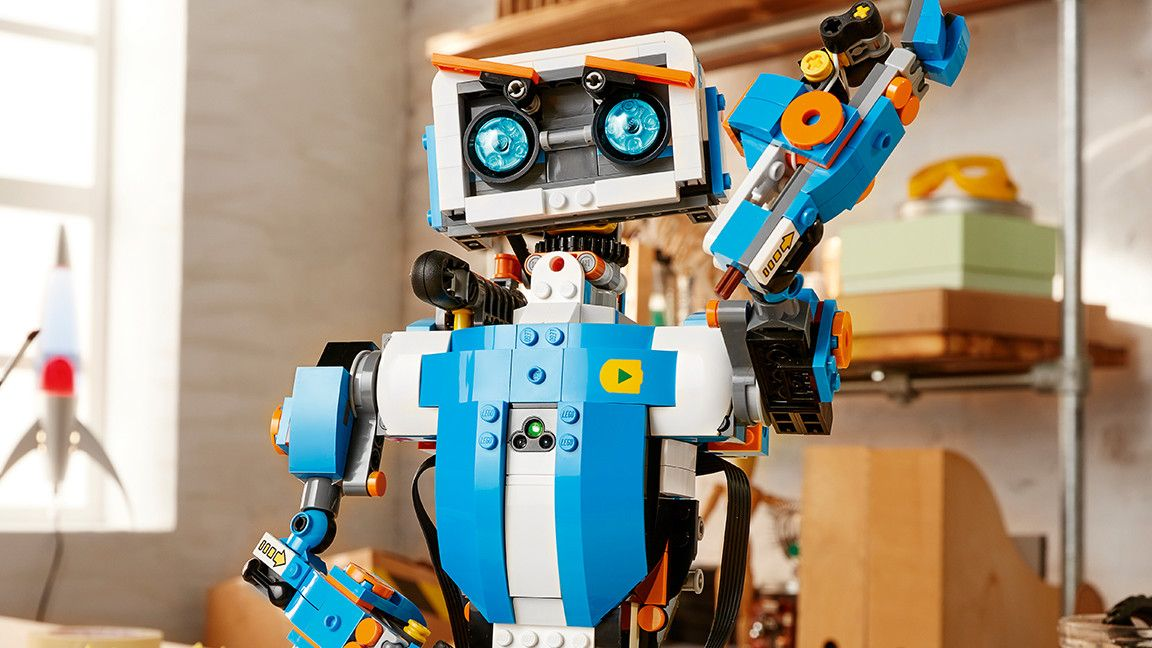
\includegraphics[width=0.8\textwidth]{07_vernie.jpg}};
                \node (led) [
                    circle,
                    draw = textColor,
                    ultra thick,
                    minimum size = 0.8cm,
                    yshift = -1.15cm,
                    xshift = -0.5cm,
                ] {};
    
                \node (text) [
                    rectangle,
                    xshift = -3cm,
                    yshift = 1.5cm,
                ] {\textbf{LED}};
    
                \draw[arrow, ultra thick] (text) to[bend right] (led);
    
            \end{tikzpicture}
    
            \caption{Position of \ac{LED} on the Vernie robot.}
            \label{fig:vernie}
        \end{figure}

        The \textsf{lego-boost-browser} library can send commands to Vernie to change the \ac{LED} color (Figure~\ref{fig:vernie}) or activate the two motors for locomotion. A publisher is created which simply publishes every second a different \ac{LED} color as a string from the acceptable list of colors by Vernie. When these messages reach the message stacks of the respective topic (e.g. \texttt{rainbow\smallunderscore topic}), they are forwarded to the robot through \textsf{lego-boost-browser}. Figure~\ref{fig:rainbow} displays what a web page running an \ac{LED} color publisher appears like. The user would have to first connect to Vernie via bluetooth before being able to send the commands to change \ac{LED} color to the one that matches the last message published. 

        \definecolor{vernOrange}{HTML}{F28B08}
        \begin{figure}[htbp]
            \centering
            \begin{tikzpicture}
                \node (start) [
                    box,
                    xshift = -5cm,
                    minimum width = 2.5cm,
                    fill = igmrLightBlue,
                ] {\footnotesize{\textbf{CONNECT}}};
                \node (vernie) [
                    rectangle,
                ] {
\includegraphics[width=3cm]{07_vernie_happy.png}};
                \node (clear) [
                    box,
                    xshift = 5cm,
                    minimum width = 2.5cm,
                ] {\footnotesize{\textbf{DISCONNECT}}};

            \end{tikzpicture}
            \vspace{2em}

            \begin{tikzpicture}
                \node (title) [
                    rectangle, 
                    xshift = -7cm,
                    yshift = 1cm,
                ] {\textbf{Publish LED colors}};

                \node (led) [
                    circle,
                    minimum size = 0.5cm,
                    xshift = -8cm,
                    draw = textColor,
                    fill = vernOrange,
                ] {};

                \node (start) [
                    box,
                    xshift = -5cm,
                    minimum width = 2.5cm,
                    fill = igmrLightBlue,
                ] {\footnotesize{\textbf{START}}};
                \node (stop) [
                    box,
                    minimum width = 2.5cm,
                ] {\footnotesize{\textbf{STOP}}};
                \node (clear) [
                    box,
                    xshift = 5cm,
                    minimum width = 2.5cm,
                ] {\footnotesize{\textbf{CLEAR}}};
            \end{tikzpicture}
            \vspace{1em}
            
            \begin{lstlisting}[language=Bash]
Initializing...
[INFO] [1682077173.551000000] [wasm_cpp]: Context initializing.
[INFO] [1682077174.584000000] [rainbow_publisher]: Publishing: 'pink'
[INFO] [1682077175.598000000] [rainbow_publisher]: Publishing: 'purple'
[INFO] [1682077176.614000000] [rainbow_publisher]: Publishing: 'blue'
[INFO] [1682077177.633000000] [rainbow_publisher]: Publishing: 'lightblue'
[INFO] [1682077178.652000000] [rainbow_publisher]: Publishing: 'cyan'
[INFO] [1682077179.574000000] [rainbow_publisher]: Publishing: 'green'
[INFO] [1682077180.591000000] [rainbow_publisher]: Publishing: 'yellow'
[INFO] [1682077181.607000000] [rainbow_publisher]: Publishing: 'orange'
\end{lstlisting}
            \caption{Publisher sending \ac{LED} colors to the Vernie robot.}
            \label{fig:rainbow}
        \end{figure}


        To control the position of the Vernie robot, a publisher which sends \texttt{geometry\smallunderscore msgs/Twist} messages was created. These messages contain a linear and an angular vector to express the velocity in free space. To ensure compatibility with \textsf{lego-boost-browser}, a few simplifications were made. First, the robot can only move forward or backwards along the $x$-axis and rotate on the same plane, $z$-axis; thus, the only relevant values from the \texttt{Twist} message are the linear velocity $\dot{x}_{lin}$ and the angular velocity $\dot{z}_{rot}$. Since the commands sent to Vernie with \textsf{lego-boost-browser} can only be expressed in terms of motor power ($P$), from 0 to $100\%$, the linear and angular command velocities are converted with the following formula:
        
        \begin{equation}
            \hskip 5cm
            \begin{bmatrix}
                1 & -1 \\
                1 & 1
            \end{bmatrix}
            \begin{bmatrix}
                x_{lin} \\
                z_{rot}
            \end{bmatrix}
            =
            \begin{bmatrix}
                P_A \\
                P_B
            \end{bmatrix}
        \end{equation}

        Afterwards, the motor power is normalized to ensure that it does not exceed the $100\%$ limit. 
        
        With this implementation, a \ac{ROS} publisher can send command velocities by publishing a \texttt{Twist} message, then these messages are converted and forwarded to the Vernie robot to activate the motors with the desired velocities.

        \vspace{1em}
        \begin{tcolorbox}[title=Example 7]
            \begin{minipage}[t]{0.87\linewidth}
                \vspace*{0.5\baselineskip}
                A demonstration of $\mathcal{C}4$ with Vernie can be found at:
                
                \href{https://ros2wasm.dev/pages/demo04/index.html}{\textsf{https://ros2wasm.dev/pages/demo04/index.html}}

                \textsc{Note:} The Web Bluetooth \ac{API} is experimental and must be enabled manually in some browsers. Chrome is recommended.
            \end{minipage}\hfill%
            \begin{minipage}[t]{0.1\linewidth}
                \vspace{14pt}
                
\includegraphics[height=\linewidth,width=\linewidth]{qr_demo04.png}
            \end{minipage}
        \end{tcolorbox}



        \subsection{User Interaction Level 4: Intermediate}

        services and info about environment









        A depiction of Level 4 is shown in Figure~\ref{fig:ui4}

        \begin{figure}[htbp]
            \centering
            \begin{tikzpicture}
                \node (title) [
                    rectangle, 
                    xshift = -7cm,
                    yshift = 1cm,
                ] {\textbf{Service Server}};

                \node (start) [
                    box,
                    xshift = -5cm,
                    minimum width = 2.5cm,
                    fill = igmrLightBlue,
                ] {\footnotesize{\textbf{START}}};
                \node (stop) [
                    box,
                    minimum width = 2.5cm,
                ] {\footnotesize{\textbf{STOP}}};
                \node (clear) [
                    box,
                    xshift = 5cm,
                    minimum width = 2.5cm,
                ] {\footnotesize{\textbf{CLEAR}}};

            \end{tikzpicture}
            \vspace{1em}

            \begin{lstlisting}[language=Bash]
Server initializing.
[INFO] [1682083640.136000000] [rclcpp]: [server] Ready to add two ints.
[INFO] [1682083644.967000000] [rclcpp]: [server] Incoming request X: 5 Y: 8
[INFO] [1682083644.968000000] [rclcpp]: [server] Sending back response: [13]
\end{lstlisting}

            \begin{tikzpicture}
                \node (title) [
                    rectangle, 
                    xshift = -7cm,
                    yshift = 1cm,
                ] {\textbf{Service Client}};

                \node (start) [
                    box,
                    xshift = -5cm,
                    minimum width = 2.5cm,
                    fill = igmrLightBlue,
                ] {\footnotesize{\textbf{START}}};
                \node (stop) [
                    box,
                    minimum width = 2.5cm,
                ] {\footnotesize{\textbf{STOP}}};
                \node (clear) [
                    box,
                    xshift = 5cm,
                    minimum width = 2.5cm,
                ] {\footnotesize{\textbf{CLEAR}}};
            \end{tikzpicture}

            \begin{lstlisting}[language=Bash]
Client initializing.
[INFO] [1682083643.384000000] [rclcpp]: [client] add_two_ints_client X Y
[INFO] [1682083643.645000000] [rclcpp]: [client] Send request X: 5  Y: 8
[INFO] [1682083646.101000000] [rclcpp]: [client] Sum: 13
\end{lstlisting}

            \caption{Service server and client interacting on the browser.}
            \label{fig:ui4}
        \end{figure}




        \begin{tcolorbox}[title=Example 8]
            \begin{minipage}[t]{0.87\linewidth}
                \vspace*{0.5\baselineskip}
                A demonstration of an \textit{intermediate} user interface ($\mathcal{I}4$) can be found at 
                
                \href{https://ros2wasm.dev/pages/demo05/index.html}{\textsf{https://ros2wasm.dev/pages/demo05/index.html}}
            \end{minipage}\hfill%
            \begin{minipage}[t]{0.1\linewidth}
                \vspace*{0pt}
                
\includegraphics[height=\linewidth,width=\linewidth]{qr_demo05.png}
            \end{minipage}
        \end{tcolorbox}


    
